\documentclass[letterpaper,11pt]{article}
\usepackage[margin=1in]{geometry}
\usepackage{natbib}
% \bibliographystyle{unsrtnat}
\usepackage{tabularx} % extra features for tabular environment
\usepackage{amsmath}  % improve math presentation
\usepackage{graphicx} % takes care of graphic including machinery
% \usepackage{cite} % takes care of citations
\usepackage[final]{hyperref} % adds hyper links inside the generated pdf file
\usepackage{longtable}
\usepackage{xcolor}
\usepackage{lineno}
\linenumbers

% ------------------------------------------------------------------------
\newcommand{\myCheckBox}{\CheckBox[width=0.8em,bordercolor={0.65 0.79 0.94},height=0.8em]}
\newcommand{\Hydro}     {H$_2$}
\newcommand{\dC}        {$^\circ$C}
\renewcommand{\arraystretch}{1.3}

% ------------------------------------------------------------------------

\begin{document}

\title{\textbf{LAr Filter Regeneration Procedure}}
\author{Yun-Tse Tsai}
\date{\today}

\maketitle

%-------------------------------------------------------------------
\underline{General steps:}
\begin{enumerate}
\setlength\itemsep{-0.2em}
\item Preheat the LAr filter to 175 -- 180{\dC} with ultra high purity Ar gas at 160~slpm 
($\sim$6.7~scfm on the flowmeter).  
It takes about 3~hours.  
Regarding the voltage of the gas heater, you can start with 55~V at the variac and bump it 
to 100 -- 110~V after everything is stable for 10~minutes.  
You can stop preheating when the bottom thermocouple reaches $\sim$145{\dC}.
Currently we are using the ultra high purity Ar from the gas port of the LAr dewar, 
because a huge amount of gas Ar is needed.
\item Use 1 -- 2\% {\Hydro} balanced with Ar to regenerate the LAr filter.  
Keep the temperature between 175 and 225{\dC}.  
With the flow rate of 80~slpm ($\sim$3.3~scfm on the flowmeter), we expect to use 5 gas cylinders, 
each takes about 1.25 hours.  
You can keep the voltage of the gas heater between 55 -- 75~V (at the variac).
\item Cool down the system with ultra high purity Ar gas.  
This take $\sim$80~minutes and you will sort of uniformly ramp down the voltage of 
the gas heater from 65~V to 20~V.
\end{enumerate}

%-------------------------------------------------------------------
\underline{Time to stop regeneration:}
\begin{itemize}
\setlength\itemsep{-0.2em}
\item Humidity plateaus.  Better plateaus at 0.02\%.
\item 5 hours of 2\% {\Hydro} gas at 80~slpm ($\sim$3.3~scfm on the flowmeter).
\item Temperature in the LAr filter does not rise anymore.
\end{itemize}

%-------------------------------------------------------------------
\underline{Safety:}
\begin{itemize}
\setlength\itemsep{-0.2em}
\item All the doors of the LNTF hut have to be open.
\item The intake fan has to be turned on.
\item The oxygen deficiency sensor and monitor (ODM) have to be checked.
\item The pressure in the LAr filter is shown on PG3.
\item The gas flow has to be greater than 2~scfm (marked on the flowmeter) to prevent the heater 
from getting too hot.
\item The gas heater power cord is plugged into the heater engineering control (EEIP approved), 
which shut down the power if the temperature
of the gas heater exceeds the preset value, 355{\dC}.  
The shut-down temperature can be set at the detector control GUI (Ignition),
and the gas heater temperature is displayed in the same page.
\item When sealed, the pressure of the LAr filter and gas pipe should not exceed 150~psig.
The pressure relief valve on the LAr filter will open at $\sim$150~psig,
while the pressure relief valves along the pipe will open at 150 -- 200~psig.
\item If seeing smoke or smelling something unusual, shut down the variac power supply (heater) 
and investigate.
\end{itemize}

%-------------------------------------------------------------------
\underline{Technical notes:}
\begin{itemize}
\setlength\itemsep{-0.2em}
\item V3, V5, V7, V9, V16/V17, V19 isolate the LAr filter.  
During the regeneration, V3 and V5 should be always closed.  
V17 is a metal valve, which will be always open.
We will rely on V16 and V19 to 
isolate the LAr filter, instead of V17.
However, we close V17 after regeneration to prevent cold Ar from entering
the gas heater when filling LAr.
\item V16, V20, V21, V22, V24, V25 are diaphrame valves and are not adjustable.
When opening them, make a full open.
Use Reg1/2/3 and V19 to control the flow rate.
\item The Ar gas flows from the gas port of the LAr dewar, Reg3, V20, V16, HT1, V17, into the LAr filter, 
and vents from V19, FC1, outside the LNTF hut along the venting pipe, as shown in 
Fig.~\ref{fig:ArFlow}.
\item The 2\%{\Hydro}+Ar gas flows from the gas cylinders, Reg1/2, V26/V27, V22, V16, HT1, V17, 
into the LAr filter, 
and vents from V19, FC1, outside the LNTF hut along the venting pipe, 
as shown in Fig.~\ref{fig:H2Flow}.
\item The vacuum vessel surrounding the LAr filter should be evacuated from V4 all the time 
during regeneration.  
The pressure can be read from PG6.
\item Control Reg1/2/3 and V19 carefully to avoid compromising the LAr filter.  
We want the LAr filter to have pressure 
greater than the atmosphere so that the air won't diffuse in, but not too overpressurized.  
16 -- 35~psia in the LAr filter is good.
% {\color{orange} We would like to get rid of V17 and V18, but if they are needed in this process, 
% please follow up.}
\item The pressure at the outlet of Reg3 and in the LAr filter should be very close to each other,
because the pressure drop along the inlet line is small.
\item The pressure at the outlet of Reg1/2 is a few psi higher then the pressure in the LAr filter,
which corresponds to the pressure drop along the inlet line. 
\item We should always keep the gas flow (Ar or 2\%{\Hydro}+Ar) between 2 and 6.7~scfm 
(marked on the flowmeter).
\item Maintain the catalyst temperature between about 175{\dC} and 225{\dC}.
\item Do NOT exceed 225{\dC}, even though 250{\dC} may be tolerated.
% \item If we keep the gas flow at 6.7~scfm Air, a gas cylinders should be finished in about an hour.
\item The temperature of the hot gas and heater body may increase while the voltage 
from the variac power supply is fixed.  
It is owing to the drop of the gas flow.  We can adjust Reg1/2 to cope with this situation.
This happens all the time with the 2\%{\Hydro}+Ar cylinders and we should keep an eye on 
these parameters.
\item The humidity sensor operates between -20{\dC} and 50{\dC}.
With the Ar flow rate of 160~slpm ($\sim$6.7~scfm on the flowmeter), the hot Ar gas likely 
still has higher temperature than 50{\dC} when it arrives the humidity sensor.
The humidity sensor will show 0\% all the time in this case.
It will start functioning when the temperature drops.
We can turn off the gas heater or lower the flow rate to obtain colder gas when we need to
check the humidity.
(Modification is being planned.)
\item The LED light on the gas heater control may be broken.  The controlling part 
should be functional, and you just have to follow the labels for the toggle switch.
\item The torque for V17 is 4~foot-pound, 3/4" socket.
% \item The torque for V18 is 21.7 foot-pound, 3/4" socket (not needed, just FYI).  
% Need different torque wrenches for V17 and V18 typically.
\end{itemize}

%-------------------------------------------------------------------
% P&ID
\clearpage
\begin{figure}[htb]
\begin{center}
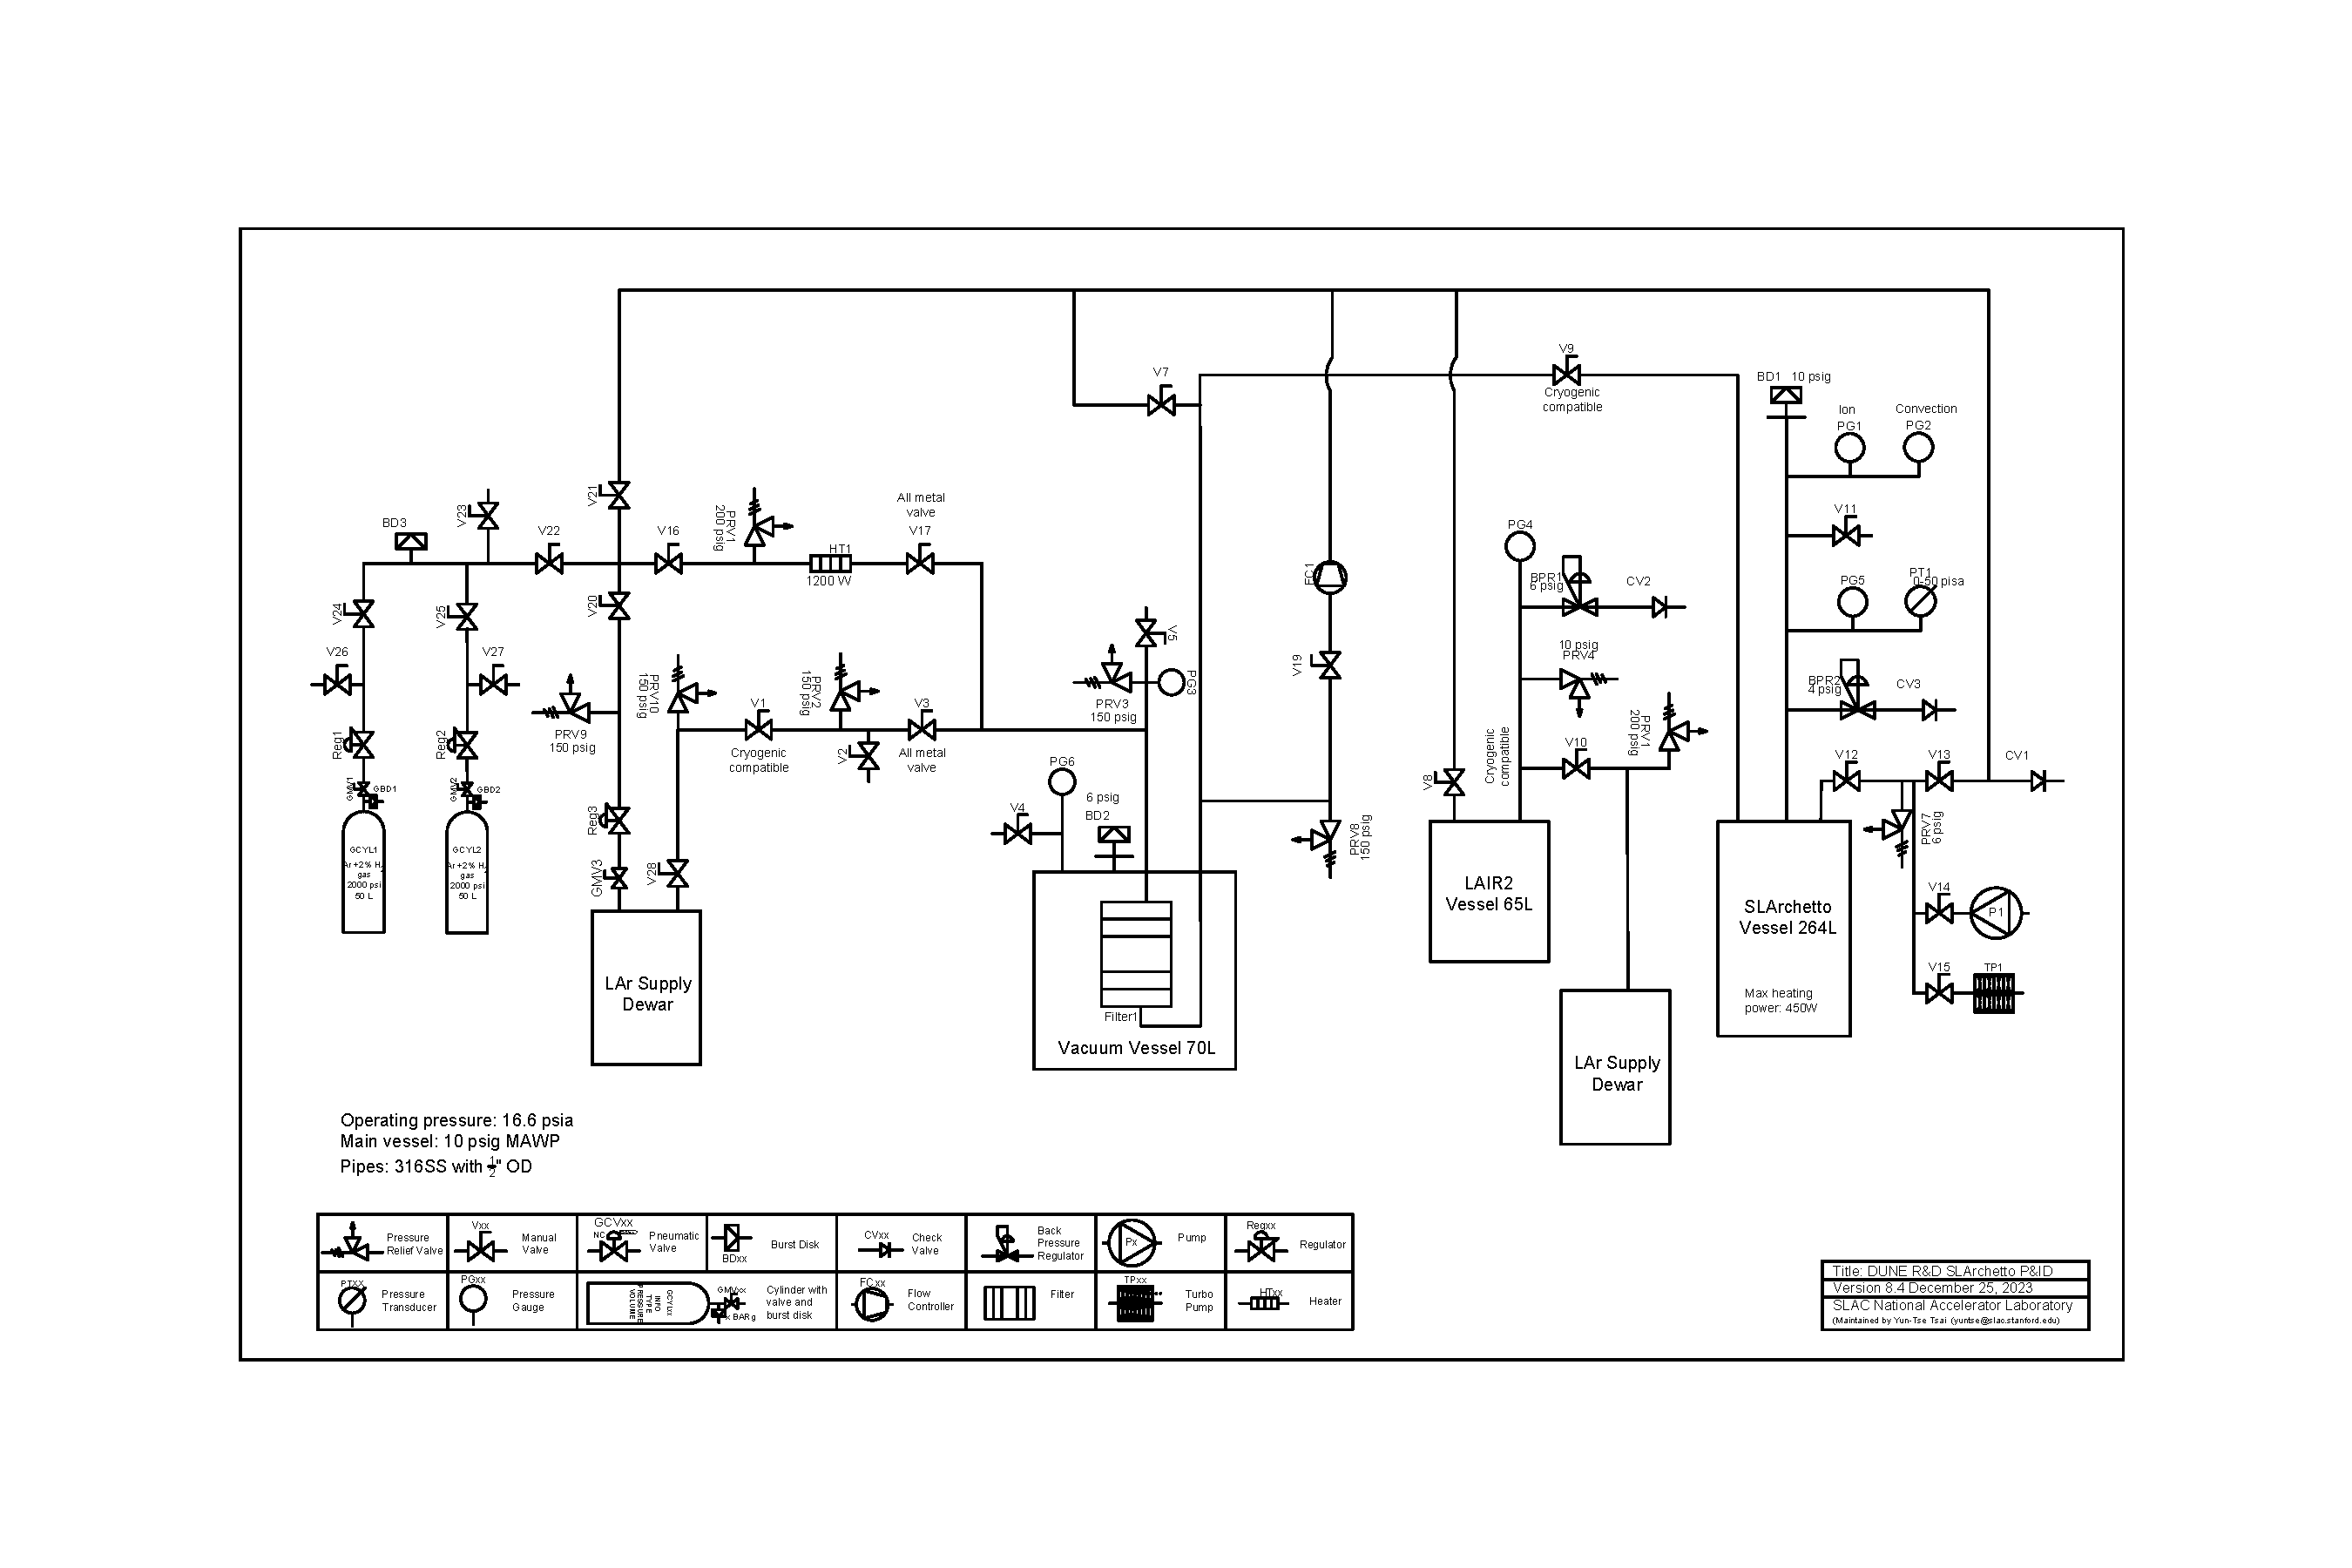
\includegraphics[angle=90,origin=c,height=7.3in]{fig/PIDv8.4.pdf}
\caption{P\&ID}
\label{fig:PID}
\end{center}
\end{figure}
%-------------------------------------------------------------------
%-------------------------------------------------------------------
% Gas flow: Ar
\clearpage
\begin{figure}[htb]
\begin{center}
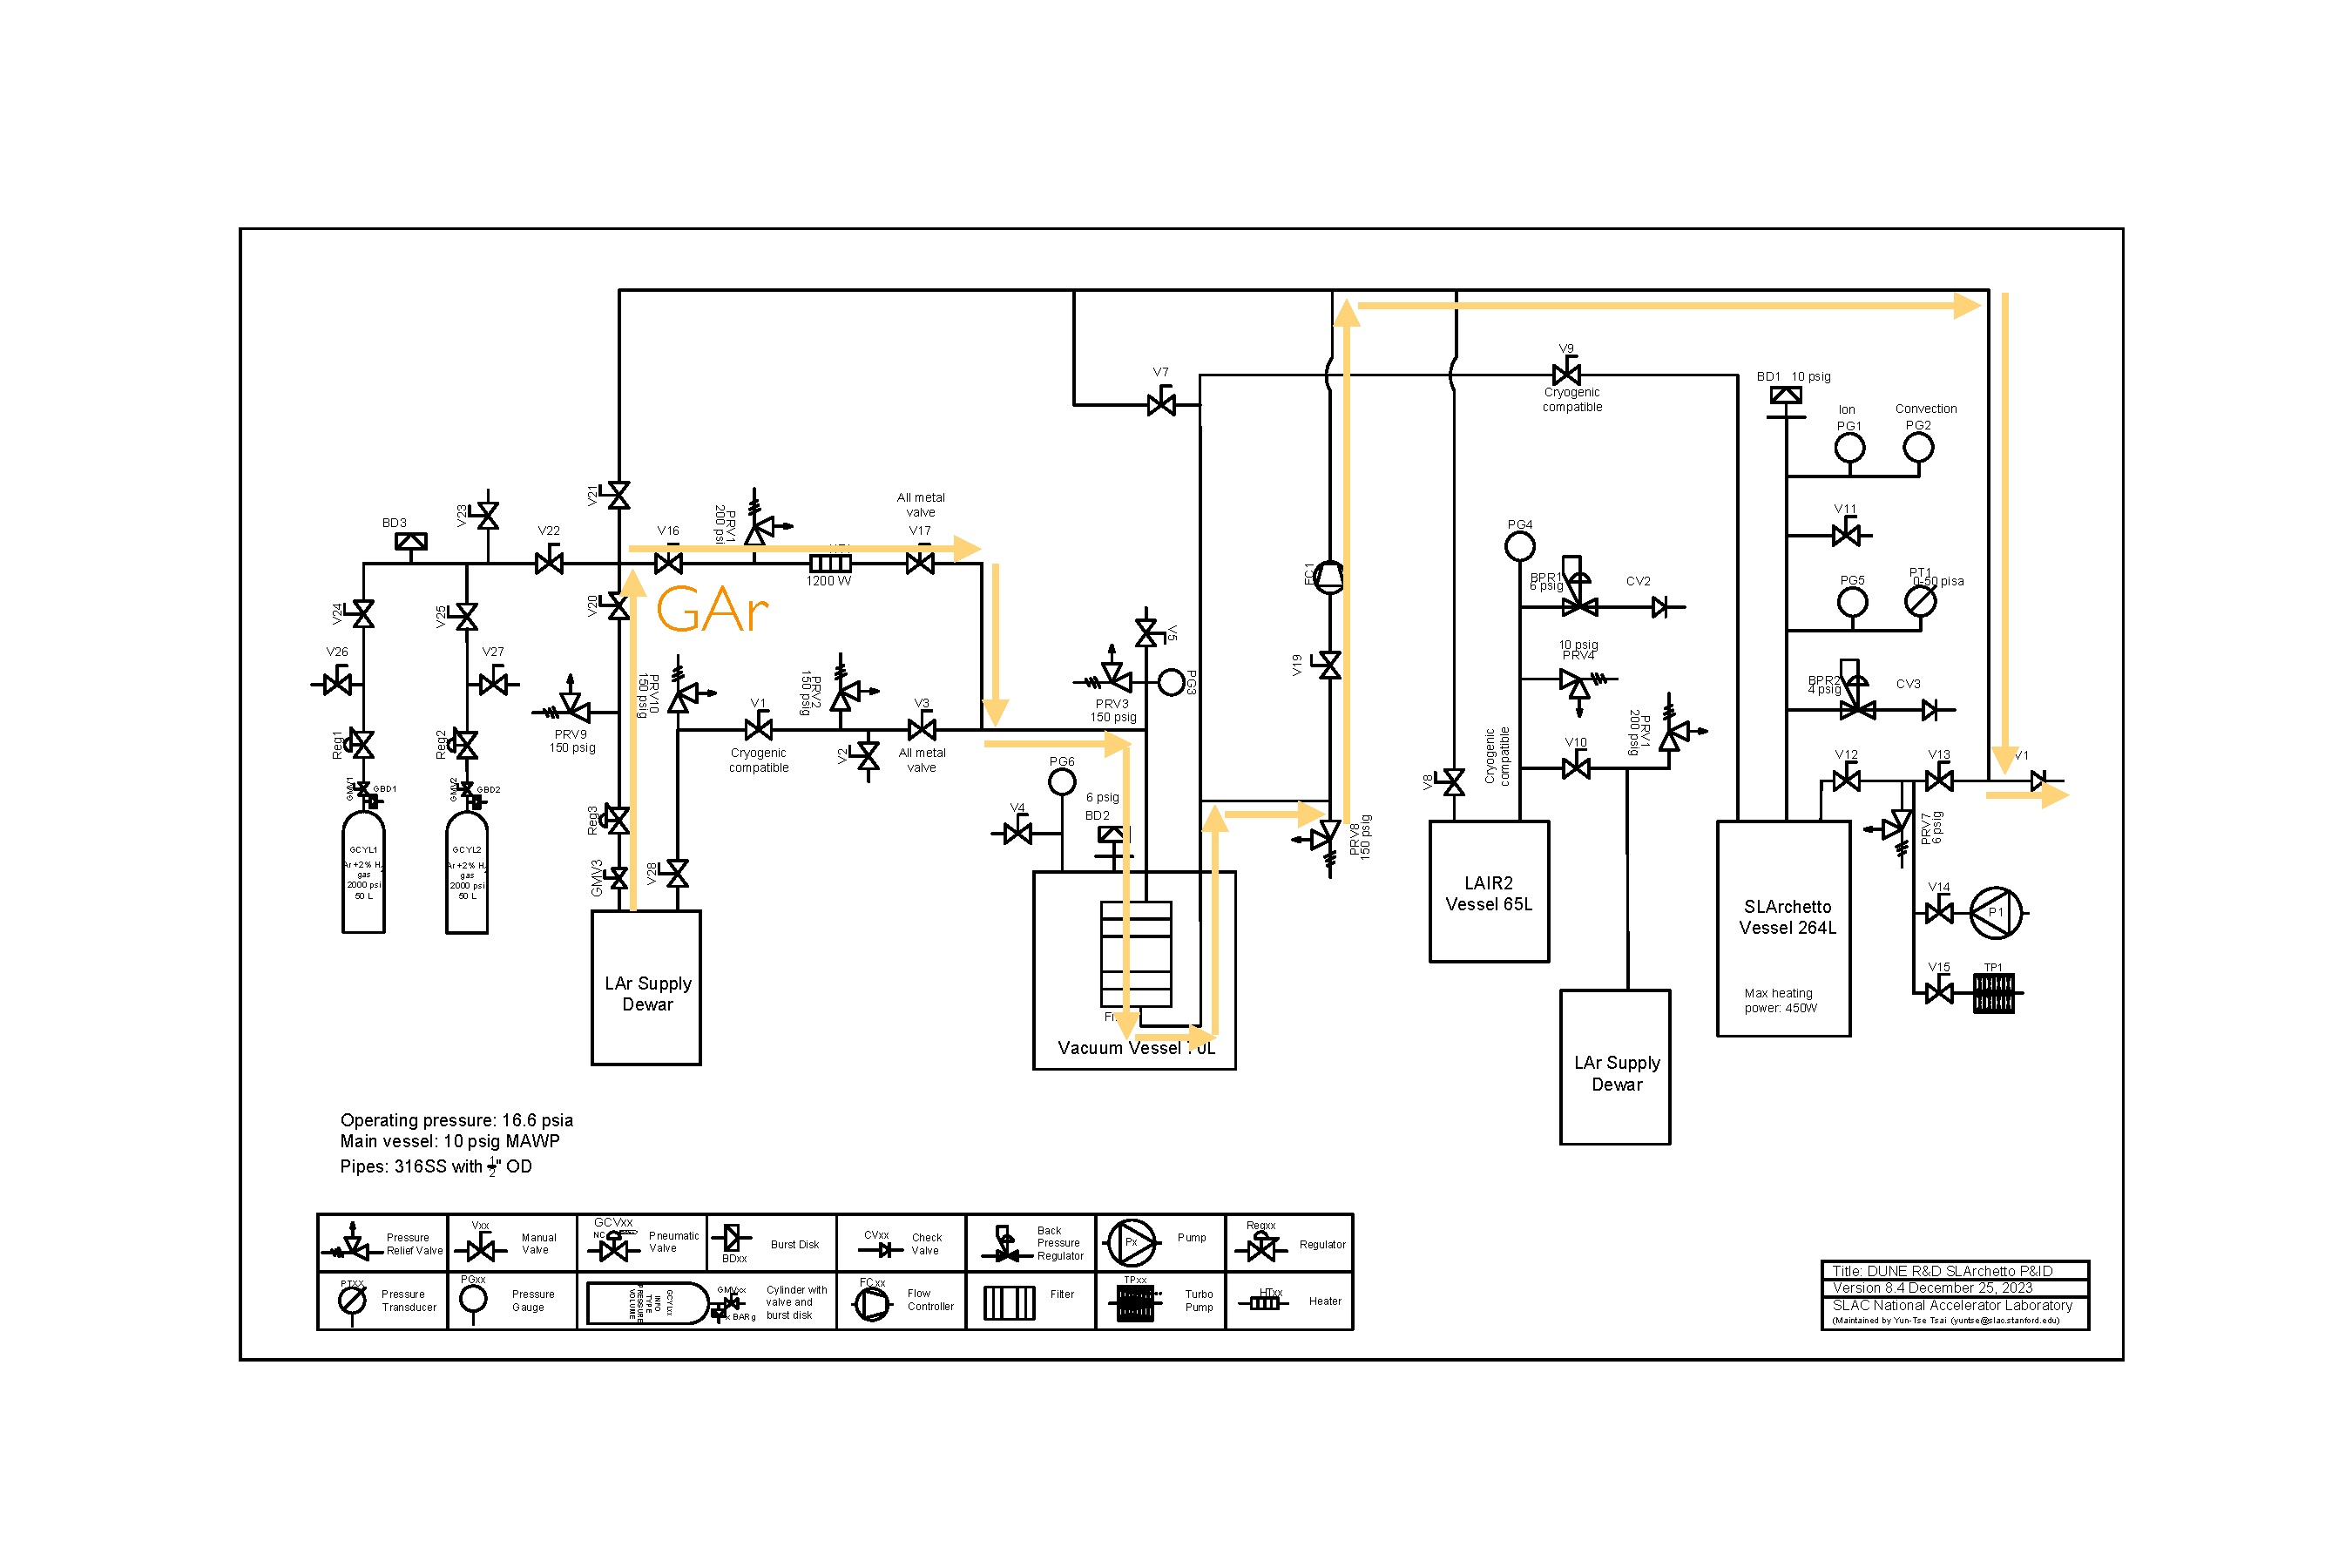
\includegraphics[angle=90,origin=c,height=7.3in]{fig/RegenerationAr_PIDv8.4.pdf}
\caption{Gas flow direction: Ar gas}
\label{fig:ArFlow}
\end{center}
\end{figure}
%-------------------------------------------------------------------
%-------------------------------------------------------------------
% Gas flow: H2+Ar
\clearpage
\begin{figure}[htb]
\begin{center}
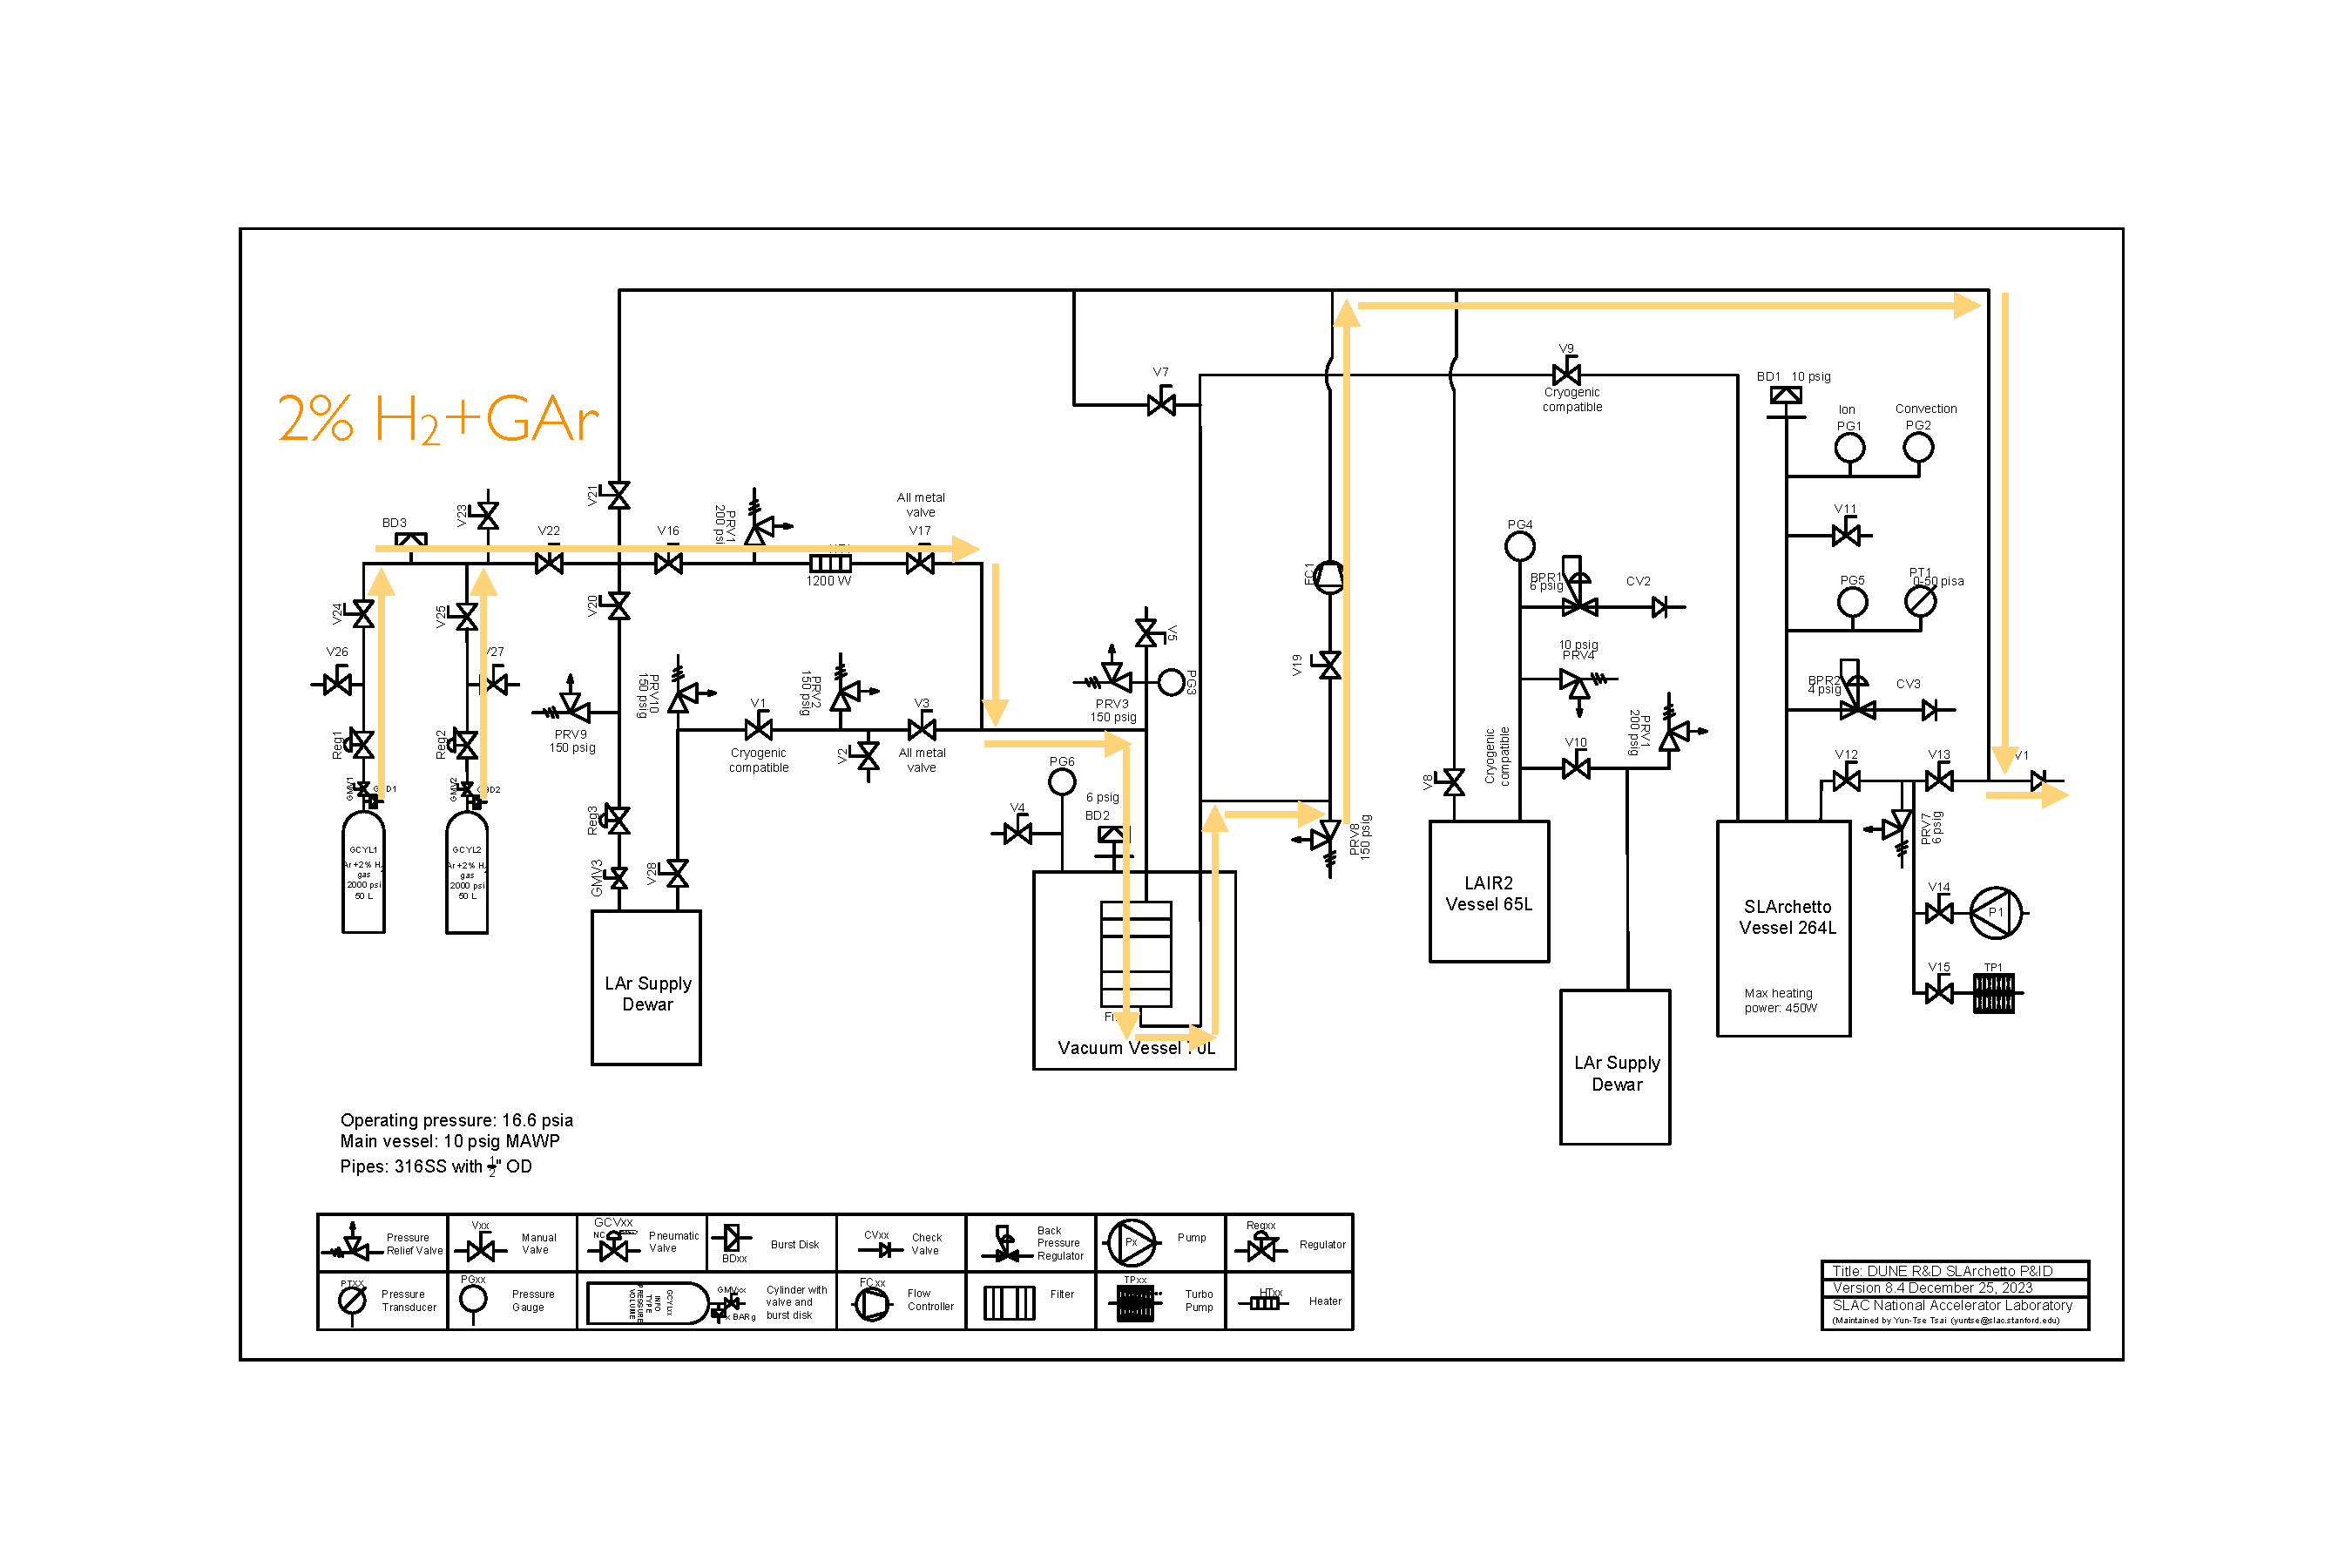
\includegraphics[angle=90,origin=c,height=7.3in]{fig/RegenerationH2_PIDv8.4.pdf}
\caption{Gas flow direction: 2\%{\Hydro}+Ar gas}
\label{fig:H2Flow}
\end{center}
\end{figure}
%-------------------------------------------------------------------

\clearpage
\tabcolsep=10pt
\begin{longtable}{p{0.5\textwidth}p{0.5\textwidth}}
\hline
\hline
Checklist & What to Do and Detailed Description \\
\hline
\multicolumn{2}{l}{\textbf{Readiness -- Before the Day}} \\
\myCheckBox{1 ultra high purity LAr dewar} & 
We use the gas port of the LAr because we need a lot amount of gas Ar.\\
\myCheckBox{The LAr dewar lifted in the LNTF hut} & \\
\myCheckBox{4 cylinders of Ar+2\%H$_2$ gas} & \\
\myCheckBox{The GAS port of the ultra high purity LAr dewar connected to Reg3 and then V20 with 
a copper tube} & \\
\myCheckBox{Two Ar+2\%{\Hydro} gas cylinders connected to Reg1/Reg2 and V24/V25 line} & \\
\myCheckBox{The cold insulation foam from the tubes close to the LAr filter regeneration line removed} & \\
\myCheckBox{Heater, tubes connecting the heater and the LAr filter wrapped with 
a few layers of aluminum foils} & For thermal insulation \\
\myCheckBox{Variac AC power supply and the gas heater engineering control ready} & \\
\myCheckBox{V4 connected to the scroll pump} & Prepare to evacuate the vacuum vessel \\
\myCheckBox{V4 opened} & \\
\myCheckBox{V4 opened, scroll pump on} & Evacuate the vacuum vessel \\
\myCheckBox{V3, V5, V7, V8, V9, V10, V11, V12, V16, V17, V19 closed} & \\
\myCheckBox{All the temperature and humidity sensors connected} & \\
\myCheckBox{Detector control (Ignition) set up} & Instruction: 
\url{https://docs.google.com/document/d/17dsjQEY3hDOYmxKYikNqeVWEoB0qyarqYrbijNPSBfg/edit?usp=sharing} \\
\myCheckBox{All sensors in the ``Filter Regeneration'' page online} & \\


\hline
\multicolumn{2}{l}{\textbf{Safety Checks -- Beginning of the Day}} \\
\myCheckBox{All the doors of the LNTF hut opened} & \\
\myCheckBox{Intake fan on} & The emergency button is yellow \\
\myCheckBox{Oxygen deficiency sensor in place, oxygen deficiency monitor green} & \\
\myCheckBox{HEPAs speed high} & HEPA control is in the back of the fans 
(outside the clean tent), and there are five HEPAs \\
\myCheckBox{Heat warning signs posted on the clean tent and the frame} & \\
\myCheckBox{Gas heater shutdown temperature set to 355{\dC}} & 
In the detector control system, click ``LAr Filter,'' set the value in 
``Gas heater switch off temperature''\\
\myCheckBox{Gas heater temperature alarm set to 400{\dC}} & 
In the detector control system, click ``LAr Filter,'' choose ``TC1: Gas heater'', 
enable the alarm and set the value\\

\hline
\multicolumn{2}{l}{\textbf{Preheating with Ar gas}} \\
\myCheckBox{V3, V5, V7, V9, V16, V19, V20, V21, V22, V23, V24, V25, V26, V27 closed} & \\
\myCheckBox{V17 fully opened} & Not going to use this valve to isolate the LAr filter; 
keeping them open \\
\myCheckBox{V4 opened, the connected scroll pump on} & \\
\myCheckBox{PG6 at 0 psia} & \\
\myCheckBox{Variac power supply off.  Voltage set at 0} & \\
\myCheckBox{Gas heater (HT1) plugged in to the heater engineering control, and the engineering 
control plugged into the variac power supply} & \\
\myCheckBox{The GAS port of the ultra high purity LAr dewar connected to Reg3 and then V20} & \\
\myCheckBox{Flowmeter (FC1) set to the maximum} & Not using the flowmeter to control the flow \\
\myCheckBox{Purge the air: GMV3 opened, Reg3 increased, V20, V21 opened} & 
Purge the air in the connection tube \\
\myCheckBox{V21, GMV3 closed} & Finish purging \\
\myCheckBox{V16 opened} & \\
\myCheckBox{One operator ready to open V19.  V19 closed} & \\
\myCheckBox{GMV3 opened, Reg3 increased.  PG3 at 5 -- 15~psig (20 -- 30~psia), V19 opened} 
& Start flowing Ar gas to the LAr filter\\
\myCheckBox{Gas flow $\sim$6.7~scfm, PG3 at 20 -- 35~psia, stable} & \\
\myCheckBox{Variac power supply on, the voltage increased to 55V} & Turn on the heater \\
\myCheckBox{10 minutes of stable conditions reached} & \\
\myCheckBox{Variac power supply set to 100 -- 110V} & \\
\myCheckBox{Humidity plateaued at 0.02\% for $>$~10~minutes} & Molecular sieves regenerated \\
\myCheckBox{Preheated for $>$~2~hours} & \\
\myCheckBox{TC0, 1, 2, 3 at 175 -- 180{\dC}, or TC3 $>145${\dC}} & \\
\myCheckBox{Variac power supply off.  Voltage set at 0} & Turn off the heater \\
\myCheckBox{V16, V19, V20 closed} & \\
\myCheckBox{GMV3 and Reg3 closed} & \\

\hline
\multicolumn{2}{l}{\textbf{Regenerating copper sieves}} \\
\myCheckBox{Variac power supply off.  Voltage set at 0} & \\
\myCheckBox{V26, V27, V24, V25, V23, V22, V20, V21, V16, V19 closed} & \\
\myCheckBox{V17 fully opened} & Not going to use this valve to isolate the LAr filter; 
keeping them open \\
\myCheckBox{Two Ar+2\%{\Hydro} gas cylinders connected to Reg1/Reg2 and V24/V25 line} & \\
\myCheckBox{Purge the air: GMV1 opened, Reg1 increased, V24, V23 opened} & 
Purge the air in the connection tube until the V22 location for the first time \\
\myCheckBox{GMV1, V23 closed} & Finish purging \\
\myCheckBox{V22, V16 opened} & \\
\myCheckBox{One operator ready to open V19.  V19 closed} & \\
\myCheckBox{GMV1 opened, Reg1 increased.  PG3 at 5 -- 15~psig (20 -- 30~psia), V19 opened} & \\
\myCheckBox{Gas flow between 50 and 160~slpm (Ar), or between 2.2 and 6.7~scfm (marked as Air).  
Preferably at 3.5~scfm Air.
PG3 (LAr filter) at 5 --20~psig (20 -- 35~psia).  The outlet of Reg1/2 at 20 -- 40~psig.} & 
Usually V19 is not widely open. \\
\myCheckBox{Variac power supply on, the voltage increased to 55 -- 75~V} & Turn on the heater \\
\myCheckBox{Temperature in the LAr filter kept at 175 -- 225{\dC}} & 
Should the temperature exceed 225{\dC} anywhere in the bed, switch to {\Hydro}-free gas and 
turn off the gas heater power supply until the hot zone cools back down to 200 -- 210{\dC}, 
then resume feeding the {\Hydro} gas mixture and turn on the gas heater power supply \\

\multicolumn{2}{l}{\textbf{Gas cylinder transition}} \\
\myCheckBox{The other gas cylinder (GCYL2) connected before the operating one (GCYL1) finishes} & 
or vice versa \\
\myCheckBox{Purge the connection line: GMV2 open, Reg2 open, V27 open} & 
Purge the air until the V25 location.  Can also evacuate from V27 instead of purging.  
When connecting to a pump, need to install a PRV (can be a KF cap) so that the pump
will not risk to encounter high pressure. \\
\myCheckBox{GMV2, V27 closed} & Finish purging \\
\myCheckBox{V22, V16 opened} & \\
\myCheckBox{One operator available to adjust V19 all the time, keeping PG3 at 5 -- 15~psig 
(20 -- 30~psia)} & \\
\myCheckBox{The operating cylinder has the pressure of $\sim$300~psig} & \\
\myCheckBox{V24 closed. GMV2 opened, V25 opened, Reg2 increased} & Transition swiftly.  
\textbf{If no gas flow, turn off the gas heater.} \\
\myCheckBox{PG3 at 5 -- 15~psig (20 -- 30~psia)} & \\
\myCheckBox{Replaced the empty cylinder with a full one} & \\

\multicolumn{2}{l}{\textbf{Finishing the copper seive regeneration}} \\
\myCheckBox{The temperature of the all catalyst bed stable or subsiding} & \\
\myCheckBox{Humidity plateaued at 0.02\% for $>$~10~minutes} & Copper sieves regenerated \\
\myCheckBox{Variac power supply off.  Voltage set at 0} & Turn off the gas heater \\
\myCheckBox{V22, V16, V19 closed} & \\
\myCheckBox{GMV1 and Reg1 closed, V24/V25 closed} & \\


\hline
\multicolumn{2}{l}{\textbf{Completion; cooling down}} \\
\myCheckBox{Variac power supply off.  Voltage set at 65~V} & \\
\myCheckBox{V16, V19, V20, V21, V22, V23, V24, V25, V26, V27 closed} & \\
\myCheckBox{V17 fully opened} & Not going to use this valve to isolate the LAr filter; 
keeping them open \\
\myCheckBox{The GAS port of the ultra high purity LAr dewar connected to Reg3 and then V20} & \\
\myCheckBox{Purge the air: GMV3 opened, Reg3 increased, V20, V21 opened} & Purge the air in the 
connection tube \\
\myCheckBox{V21, GMV3 closed} & Finish purging \\
\myCheckBox{V16 opened} & \\
\myCheckBox{One operator ready to open V19.  V19 closed} & \\
\myCheckBox{GMV3 opened, Reg3 increased.  PG3 at 5 -- 15~psig (20 -- 30~psia), V19 opened} 
& Start flowing Ar gas to the LAr filter\\
\myCheckBox{Gas flow $\sim$6.7~scfm, stable} & \\
\myCheckBox{Variac power supply on, the voltage slowly decreased to 20~V} & Turn on the heater \\
\myCheckBox{Temperature in the LAr filter decreased to $\sim$35{\dC}} & \\
\myCheckBox{Variac power supply off.  Voltage set at 0} & Turn off the heater \\
\myCheckBox{V16, V19 closed} & \\
\myCheckBox{GMV1 and Reg1 closed, V20 closed} & \\
\myCheckBox{V4 closed, scroll pump off} & \\

\hline
\multicolumn{2}{l}{\textbf{Power disconnection, cleanup}} \\
\myCheckBox{V17 closed} & Use a torque wrench with a 3/4" socket.  The torque is 4 foot-pound. \\
\myCheckBox{The gas heater power supply disconnected and stored} & \\
\myCheckBox{The power of the scroll pump disconnected} & \\
\myCheckBox{Intake fan off} & The emergency button is red \\
\myCheckBox{LNTF doors closed} & \\
\myCheckBox{The empty gas cylinders disconnected, moved to the empty cylinder rack and chained 
appropriately} & \\
% \myCheckBox{Disconnect the LAr dewar} & \\
\myCheckBox{The heat warning signs removed (after the system cools down)} & \\

\hline
\hline
\end{longtable}

\end{document}
